\documentclass[a4paper]{article}
\usepackage{luatexja}            % LuaTeX用の日本語パッケージ
\usepackage{fontspec}
\setmainfont{IPAexMincho}       % 日本語フォントを指定
\usepackage{xcolor}              % 色の定義用パッケージ
\usepackage{listings}            % コード表示用パッケージ
\usepackage{bardiag}
\usepackage{pstricks}
\usepackage{graphicx}

\begin{document}

    \title{交通事故発生率}
    \author{松本 侑万}
    \date{2025}
    \maketitle

    \section{死傷者数の推移}

    \begin{figure}[h]
        \centering
        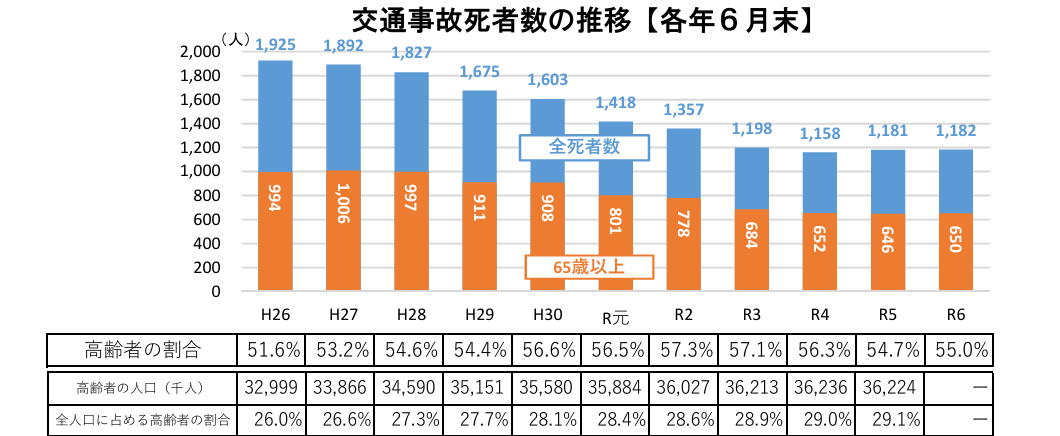
\includegraphics[scale = 0.7]{jiko.png}
        \caption{交通事故発生率}
        \label{fig:交通事故発生率}
    \end{figure}

    令和6年までのデータでは、特に65歳以上の高齢者の死亡事故が多いことが示されています。\\
      
    \begin{figure}[h]
        \centering
        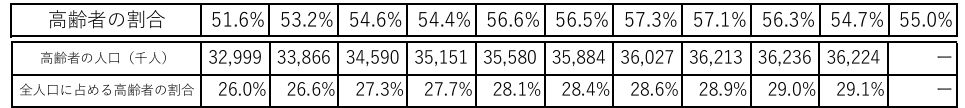
\includegraphics[scale = 0.7]{jiko2.png}
        \caption{高齢者の割合}
        \label{fig:交通事故発生率}
    \end{figure}

    この層では歩行中に自己に遭遇するケースが最も多く、年齢別で見ると高齢者が事故の大きな割合を占めています。\\




\end{document}     
